%%%%%%%%%%%%%%%%%%%%%%%%%%%%%%%%%%%%%%%%%%%%%%%%%%%%%%%%%%%%%%%%%%%%%
% LaTeX Template: Project Titlepage Modified (v 0.1) by rcx
%
% Original Source: http://www.howtotex.com
% Date: February 2014
% 
% This is a title page template which be used for articles & reports.
% 
% This is the modified version of the original Latex template from
% aforementioned website.
% 
%%%%%%%%%%%%%%%%%%%%%%%%%%%%%%%%%%%%%%%%%%%%%%%%%%%%%%%%%%%%%%%%%%%%%%

\documentclass[12pt]{report}
\usepackage[a4paper]{geometry}
\usepackage[myheadings]{fullpage}
\usepackage{fancyhdr}
\usepackage{lastpage}
\usepackage{graphicx, wrapfig, subcaption, setspace, booktabs}
\usepackage[T1]{fontenc}
\usepackage[font=small, labelfont=bf]{caption}
\usepackage{fourier}
\usepackage[protrusion=true, expansion=true]{microtype}
\usepackage{sectsty}
\usepackage{url, lipsum}
\usepackage{listings}
\usepackage[utf8]{inputenc}
\usepackage[italian]{babel}

\lstset{
  basicstyle=\ttfamily,
  columns=fullflexible,
  frame=single,
  breaklines=true,
}

\newcommand{\HRule}[1]{\rule{\linewidth}{#1}}
\onehalfspacing
\setcounter{tocdepth}{5}
\setcounter{secnumdepth}{5}

%-------------------------------------------------------------------------------
% HEADER & FOOTER
%-------------------------------------------------------------------------------
\pagestyle{fancy}
\fancyhead{}
\setlength\headheight{15pt}
\fancyhead[L]{Intelligenza Artificiale e Laboratorio}
\fancyhead[R]{Universit\`a degli Studi di Torino}
%\fancyfoot[R]{Page \thepage\ of \pageref{LastPage}}
%-------------------------------------------------------------------------------
% TITLE PAGE
%-------------------------------------------------------------------------------

\begin{document}

\title{ \normalsize \textsc{}
        \\ [2.0cm]
        \HRule{0.5pt} \\
        \LARGE \textbf{\uppercase{Intelligenza Artificiale e Laboratorio: \\ Prolog}}
        \HRule{2pt} \\ [0.5cm]
        \normalsize \today \vspace*{5\baselineskip}}

\date{}

\author{
        Andrea Forgione: 809240 \\ 
        Arthur Capozzi:  802586 \\
        Leonardo Zanchi: 800935}

\maketitle
\tableofcontents
\newpage

%-------------------------------------------------------------------------------
% Section title formatting
\sectionfont{\scshape}
%-------------------------------------------------------------------------------

%-------------------------------------------------------------------------------
% BODY
%-------------------------------------------------------------------------------

\chapter*{Introduzione}
Questa \`e la relazione riguardante l'implementazione in prolog di alcune strategie di ricerca.
La relazione \`e strutturata in tre parti: nella prima verranno elencati i due domini di applicazione, nella seconda saranno presentate le strategie, mentre nella terza risultati che queste hanno portato.

\chapter{Domini di applicazione}
I domini scelti tra quelli proposti in questa relazione sono due: la metropolitana di Londra e il mondo dei blocchi.
In questo capitolo se ne darà una descrizione cos\`i che il lettore possa farsi un'idea di quella che fosse la richiesta.

\section{Metropolitana di Londra}

\begin{figure}[!ht]
   \centering
   \includegraphics[width=1\textwidth]{immagini/metro.jpg}
   \caption{}
   \centering
   \label{label: linea della metropolitana di Londra}
\end{figure}

Il primo dominio consiste in una rappresentazione ridotta del funzionamento della metropolitana della capitale inglese.
Ridotta perché non tutte le linee sono prese in considerazione e non tutte le fermate presenti sono riportate.
La richiesta in questo dominio è trovare i cammini che portino ad una certa stazione della metropolitana a partire da un'altra fermata di questa.\\
La descrizione formale del dominio è contenuta nel file \emph{tube06-07.pl}.
Sono possibili solo tre azioni: \emph{sali/2},\emph{ scendi/1} e \emph{vai/4}.
L'azione \emph{sali/2} ha arit\`a due e necessit\`a della \emph{Linea} e della \emph{Direzione}.
L'azione \emph{scendi/1} ha arit\`a uno e necessit\`a della sola \emph{Stazione}.
L'azione \emph{vai/4} ha arit\`a e necessit\`a della \emph{Linea}, della \emph{Direzione}, della \emph{Stazione di partenza} e della \emph{Stazione di arrivo}.
La possibilit\`a di svolgere un'azione \`e espressa dalla regola \emph{applicabile}, mentre la reale applicazione dell'azione è svolta dalla regola \emph{trasforma}.\\
Il fatto \emph{percorso/3} rappresenta la nozione di linea; ha arit\`a tre e viene specificato il nome della \emph{Linea}, la \emph{Direzione} ed infine una lista contentente la \emph{Lista delle fermate}. Attraverso un regola \emph{percorso}, invece, sono specificate le direzione inverse delle fermate della metropolitana.
La regola \emph{tratta/4} consente di trovare la fermata successiva di una certa stazione.\\
Una serie di fatti \emph{stazione/3} rappresentano le stazioni presente nel modello metropolitana qui riportato; ha arit\`a tre e specifica il nome della \emph{Stazione} e la sua posizione.
La regola \emph{fermata/2} rappresenta la stazione all'interno del percorso.
Due fatti \emph{iniziale/1} e \emph{finale/1} specificano la stazione di partenza e la stazione di arrivo ricercata. Entrambi hanno arit\`a uno.

\section{Mondo dei blocchi}

Il secondo dominio scelto è quello del mondo dei blocchi. \`E un dominio ampiamente citato in letteratura in cui un numero variabile di blocchi si trovano disposti su di un tavolo. Possono trovarsi direttamente poggiati sul tavolo, oppure sopra ad un altro blocco. Un blocco può essere spostato solo se non ha su di se altri blocchi.I blocchi devono essere spostati fino ad arrivare alla configurazione finale voluta.
La descrizione formale del problema si trova all'interno del file \emph{blocchiord12.pl}.\\
Sono possibili quattro azioni differenti: \emph{pickup/1}, \emph{putdown/1}, \emph{stack/1} e \emph{unstack/1}.
Tutte le azioni hanno arit\`a uno, dove viene specificato il blocco su cui compiere l'azione.
Anche in questo dominio sono presenti due regole: \emph{applicabile/2} e \emph{trasforma/3}. Nel primo caso viene specificata l'azione da fare e lo stato in cui viene compiuta tale azioni; nel secondo caso, invece, si specifica l'azione da realizzare, lo stato di partenza e quello di arrivo.
L'azione \emph{applicabile} viene utilizzata per verificare la possibilit\`a o meno di applicare l'azione scelta, mentre \emph{trasforma} realizza l'azione portando il sistema nel nuovo stato.\\
Una serie di fatti \emph{block/1} rappresentato l'entit\`a del blocco all'interno del nostro modello.
Infine, tre fatti specificano lo stato iniziale del sistema, indicato con \emph{iniziale/1} e lo stato finale, con \emph{finale/1}.\\
Per dare un'idea del funzionamento della regola \emph{applicabile} viene riportata quella che fa riferimento all'azione \emph{unstack/2}.

\begin{lstlisting}[language=Prolog]
applicabile(unstack(X,Y),S):-
	block(X), block(Y), X\=Y,
	ord_memberchk(on(X,Y),S),
	ord_memberchk(clear(X),S),
	ord_memberchk(handempty,S).
\end{lstlisting}

In questo caso la regola \emph{unstack} sarà soddisfatta, e quindi l'azione \emph{unstack/2} applicabile, quando esiste il blocco \emph{X}, esiste il blocco \emph{Y}, i blocchi sono diversi tra di loro, il blocck \emph{X} si trova su \emph{Y} nello stato \emph{S}, il blocco \emph{X} è libero (non ha blocchi sopra di lui) nello stato \emph{S}, e la mano è libera nello stato \emph{S}.

\begin{figure}[!ht]
   \centering
   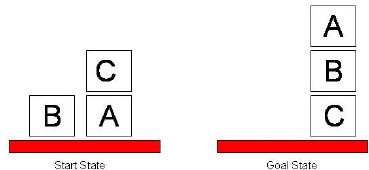
\includegraphics[width=0.7\textwidth]{immagini/blocks.png}
   \caption{}
   \centering
   \label{label: Esempio di mondo dei blocchi}
\end{figure}

\chapter{Strategie di ricerca}
In questo capitolo vengono riportate le tre strategie di ricerca richieste e i risultati ottenuti applicandole ai domini riportati nel capitolo 1.
Il capitolo è diviso in tre parti, una per ogni algoritmo implementato, e in ognuna di esse è descritto il funzionamento sui domini considerati.

\section{Iterative deepening}
\`E l'unica strategia di ricerca non informata presa in esame in questa relazione.
L'idea chiave di \emph{Iterative Deepening} (da ora \emph{IDS}) \`e quella di ri-calcolare gli elementi della frontiera piuttosto che salvarli ogni volta. Viene utilizzata una ricerca in profondit\`a limitata (\emph{Depth-bounded depth-first search}, che viene incrementata ad ogni nuova ricerca se non si giunge allo stato goal. \emph{IDS} combina i vantaggi della ricerca in ampiezza (\emph{Breadth-first}) e quelli della ricerca in profondit\`a(\emph{Depth-first}), quindi ha i requisiti modesti di memoria della \emph{Depth-first} e la completezza della \emph{Breadth-first} quando il \emph{branching factor} \`e finito. Inoltre, \`e una strategia di ricerca ottima quando il costo del cammino è una funzione monotona della profondit\`a.

\subsection{Metropolitana di Londra}
In questa sezione viene riportato l'algoritmo \emph{Iterative Deepening} applicato al dominio della metro di Londra.
Sono allegati alla relazione i relativi sorgenti, debitamente commentati, ma se ne dar\`a anche qua una decrizione dettagliata.
Riguardo il binomio \emph{IDS-metro} si fa riferimento ai file:

\begin{itemize}
\item \emph{1\_iterative\_deepening\_tube.pl}: è l'algoritmo che implementa la strategia di ricerca \emph{Iterative Deepening};
\item \emph{action\_tube.pl}: in esso è descritto il dominio, con regole e fatti.
\end{itemize}

La regola \emph{iterative\_deepening/0} \`e il punto di entrata del programma e nel corpo ha tre goal che devono essere soddisfatti affinché la regola dia come risultato \emph{true}: che esista il fatto \emph{iniziale(StartNode} e che sia vero \emph{iterative\_deepening\_search/3}. Il fatto finale semplicemente stampa la soluzione trovata.
\emph{iterative\_deepening\_search/3} \`e la regola che gestisce la chiamata alla ricerca in profondit\`a limitata. Ne esistono due versioni, la prima (indicata nel listato con il commento \%1) \`e la regola che richiama la ricerca in profondit\`a limitata, mentre la seconda (indicata nel listato con il commento \%2) si preoccupa di aggiornare la profondit\`a di ricerca nel caso in cui l'iterazione precendente di ricerca non sia andata a buon fine.
La prima, infatti, ha come parte del corpo la chiamata a \emph{dfs\_bounded/4}, cioè la ricerca in profondit\`a limitata.
La seconda, invece, ha nel corpo l'incremento della profondit\`a e la chiamata alla prima (\emph{iterative\_deepening\_search/3}) con la nuova profondit\`a.
La regola \emph{dfs\_bounded/4} (indicata con \%3) è il cuore dell'implementazione e necessita del nodo attuale, della profondit\`a di ricerca, di una lista dei nodi visitati ed infine una lista di azioni possibili su quel nodo. Nel corpo ci si accerta che:

\begin{enumerate}
\item la prondit\`a sia maggiore di zero;
\item l'azione selezionata (quella in testa alla lista \emph{[Action | OtherAction]}) sia applicabile al nodo attuale;
\item l'esecuzione dell'azione porti in un nuovo nodo;
\item il nuovo nodo trovato non appartenga alla lista dei nodi visitati (il comando \emph{member/2} deve restituire \emph{fail} come risultato, il quale verrà negato da \emph{\\\\+});
\item si aggiorna la profondit\`a riducendola di 1;
\item si chiama di nuovo la ricerca con la nuova profondit\`a a partire dal nuovo nodo, aggiornando la lista nei nodi visitati.
\end{enumerate}

La regola \emph{dfs\_bounded/4} (indicata con \%4) ha nel corpo una sola condizione per essere vera, cioè che si sia trovato lo stato finale della ricerca. Da notare l'utilizzo della \emph{CUT}, che si rende necessaria per evitare che Prolog faccia \emph{backtracking} e vada ad inficiare la soluzione trovata.

\begin{lstlisting}[language=Prolog][caption={Iterative deepening},captionpos=b]
:- use_module(action_tube).

dfs_bounded(Node, _, _, []) :- %4
	finale(Node), !.

dfs_bounded(Node, MaxDepth, Visited, [Action | OtherAction]) :- %3
	MaxDepth > 0,
	applicabile(Action, Node),
	trasforma(Action, Node, NewNode),
	\+ member(NewNode, Visited),
	NewMaxDepth is MaxDepth - 1,
	dfs_bounded(NewNode, NewMaxDepth, [Node | Visited], OtherAction).

iterative_deepening_search(StartNode, MaxDepth, PathSolution) :- %1
	dfs_bounded(StartNode, MaxDepth, [], PathSolution).

iterative_deepening_search(StartNode, MaxDepth, PathSolution) :- %2
	NewMaxDepth is MaxDepth + 1,
	iterative_deepening_search(StartNode, NewMaxDepth, PathSolution).

iterative_deepening :-
	iniziale(StartNode),
	iterative_deepening_search(StartNode, 1, PathSolution),
	write(PathSolution).
\end{lstlisting}

\subsection{Mondo dei blocchi}
In questa sezione viene riportata l'implementazione della strategia di ricerca \emph{Iterative deepening} applicata al dominio del mondo dei blocchi.
In realtà, però, dato la modularità con cui è stato scritto il programma, la parte dell'algoritmo, contenuta nel file \emph{1\_iterative\_deepening\_block.pl}, è identica a quella già vista nella sezione \emph{Iterative deepening} dedicata alla metropolitana di Londra. Per questo motivo non si riporterà in questa parte il modo in cui viene attuata la strategia.
Altri due moduli fanno parte di questa soluzione: \emph{configuration\_block} e \emph{action\_block}. Il primo contiene i fatti che definiscono i blocchi, lo stato iniziale e lo stato finale. In aggiunta, due configurazioni sono state realizzate, con numero diverso di blocchi e di conseguenza una complessità differente. Il secondo, invece, contiene la descrizione del dominio riportata nel capitolo 1, con \emph{applicabile} e \emph{transforma}.

\section{A*}
\`E un algoritmo di ricerca informata che fa uso di una euristica per stimare la distanza dal nodo attuale al nodo finale.
\emph{A*} compie una ricerca nello spazio degli stati andando ad espandere ad ogn passo il nodo appartenente alla frontiera con costo \emph{f(n)} minore. La funzione \emph{f(n)} è definita come $f(n) = g(n) + h(n)$, dove \emph{g(n)} è il costo effettivo del cammino fino al nodo \emph{n}, e \emph{h(n)} è una stima del costo del cammino dal nodo \emph{n} al nodo finale.\emph{f(n)} può essere quindi definito come il costo stimato della soluzione più conveniente che passa per il nodo \emph{n}.\\
La ricerca mediante l'algoritmo \emph{A*} trova la soluzione cercata, ma solo se l'euristica soddisfa certe condizioni:

\begin{itemize}
\item ammissibilità, cioè \emph{h(n)} non deve mai stimare per eccesso il costo per arrivare al nodo.
\item consistenza, cioè la funzione euristica deve essere monotona, $h(n) <= c(n, a, n') + h(n')$.
\end{itemize}

Le proprietà seguente garantiscono una ricerca ottima da parte di {A*}. In realtà, la consistenza è necessaria solo se la ricerca è effettuata su un grafo, mentre su un albero l'ammissibilità dell'euristica è sufficiente all'ottimalità.

\subsection{Metropolitana di Londra}
In questa sezione viene riportata l'implementazione dell'algoritmo \emph{A*} per il dominio della metropolitana di Londra.
Sono allegati alla relazione i relativi sorgenti, che sono qua riportati:

\begin{itemize}
\item \emph{3\_astar\_tube.pl} contiene l'implementazione dell'algoritmo di ricerca;
\item \emph{heuristic\_tube.pl} contiene le euristiche utilizzate per la ricerca;
\item \emph{action\_tube.pl} contiene la descrizione del dominio con regole e fatti;
\end{itemize}

In questo caso, quindi, il programma \`e stato diviso in tre moduli differenti, cos\`i da avere una maggiore versatilit\`a, permettendo di adattare velocemente ad un altro dominio la stessa strategia di ricerca.


\begin{lstlisting}[language=Prolog][caption={A*},captionpos=b]
:- use_module(action_tube).
:- use_module(heuristic_tube).

astar_search([nodo(_, _, Node, ActionsAvailable)| _], _, ActionsAvailable) :- %1
	finale(Node).

astar_search([nodo(F, G, Node, ActionsAvailable) | OtherActions], CloseNodes, PathSolution) :- %2
	member(Node, CloseNodes) -> astar_search(OtherActions, CloseNodes, PathSolution);
	expand(nodo(F, G, Node, ActionsAvailable), NextNodes),
	ord_union(OtherActions, NextNodes, Tail),
	astar_search(Tail, [Node | CloseNodes], PathSolution). 

expand(nodo(F, G, Node, ActionsAvailable), NextNodes) :-
	findall(Action, applicabile(Action, Node), ListActions),
	successor(nodo(F, G, Node, ActionsAvailable), ListActions, NextNodes)

successor(_, [], []).
successor(nodo(F, G, Node, ActionsAvailable), [Action | OtherActions], Successors) :-
	trasforma(Action, Node, NewNode),
	append(ActionsAvailable, [Action], NewActionAvailable),
	successor(nodo(F, G, Node, ActionsAvailable), OtherActions, OtherNodes),
	g(G, Node, NewNode, NewG),
	h(NewNode, NewH),
	NewF is NewG + NewH,
	ord_add_element(OtherNodes, nodo(NewF, NewG, NewNode, NewActionAvailable), Successors).

astar :-
	iniziale(Node),
	h(Node, H),
	G is 0,
	F is G + H,
	astar_search([nodo(F, G, Node, [])], [], PathSolution),
	write(PathSolution).
\end{lstlisting}

Il punto di entrata è la regola \emph{astar}, che per essere vera deve soddisfare tutti i goal del suo corpo:

\begin{itemize}
\item deve esistere il nodo \emph{iniziale(Node)};
\item deve esistere l'euristica \emph{h(Node, H)} del nodo corrente;
\item deve esistere \emph{G} uguale a zero;
\item deve esisere F uguale alla somma di \emph{G} e \emph{H};
\item \emph{astar\_search/3} deve essere true;
\item \emph{write(PathSolution)} stampa a video il cammino trovato;
\end{itemize}

La regola \emph{astar\_search/3} \`e utilizzata per la ricerca ricorsiva della soluzione. Ne esistono due, una per il caso base, e l'altra per la ricorsione.\\
La prima (indicata con \%1 nel listato) \`e vera se il nodo attuale \`e quello finale. In tal caso la ricerca \`e finita e l'algoritmo termina scrivendo il cammino trovato. Da notare come in questo caso non sia presente la \emph{CUT}, che invece era stata utilizzata nella ricerca \emph{Iterative deepening}.\\
La seconda, invece, (indicata con \%2 nel listato) \`e vera:

\begin{itemize}
\item se il nodo attuale fa parte della lista dei nodi chiusi, allora la ricerca riparte escludendo l'attuale nodo preso in esame perché già chiuso; In caso contrario, la presenza del "\emph{;}" permette di passare a valutare il secondo goal;
\item se si espande a partire dal nodo attuale;
\item se le liste dei nodi e dei vicini del nodo attuale vengono unite in nuova lista;
\item riparte la ricerca con la nuova frontiera, inserendo il vecchio nodo nella lista dei nodi chiusi e con il cammino finora percorso;
\end{itemize}
La regola \emph{expand/2} permette di espandere l'attuale nodo; nello specifico:

\begin{itemize}
\item il comando \emph{findall/3} restituisce in una lista tutte le azioni possibili dal nodo attuale;
\item \emph{successor/3} cerca i nodi raggiungibili dall'attuale nodo con le azioni individuate precedentemente;
\end{itemize}

La regola \emph{successor/3}, anche in questo caso, ha un caso base e una chiamata ricorsiva. La prima, in realtà, è semplicemente un fatto che sancisce che quel nodo non ha figli. La regola ricorsiva, invece, vale negli altri casi ed è vera se:

\begin{itemize}
\item l'azione individuata porta ad un nuovo nodo;
\item si richiama la funzione \emph{successor/3} dal nodo attuale con le restenanti azioni trovate sui nodi successivi;
\item viene calcolata la \emph{g} del nuovo nodo;
\item viene calcolata la \emph{h} dal nuovo nodo;
\item viene calcolata la nuova \emph{f} ;
\item tutti i nodi individuati vengono aggiunti alla lista dei nodi successori;
\end{itemize}

\subsubsection{Euristica della metropolitana di Londra}
L'euristica utilizzata nella metropolitana di Londra è la distanza Euclidea. Tale scelta è dovuta al fatto che la distanza euclidea è un euristica ammissibile, dato che essa rappresenta la distanza minima tra due punti.

\subsection{Mondo dei blocchi}
In questa sezione viene riportata l'implementazione della strategia di ricerca \emph{A*} per il dominio del mondo dei blocchi.
Come nel caso dell'\emph{Iterative deepening}, l'algoritmo è il medesimo utilizzato per la metropolitana di Londra.
La soluzione è divisa però in quattro blocchi, data la presenza del modulo dell'euristica:

\begin{itemize}
\item \emph{3\_astar\_block.pl} contiene regole e fatti che realizzano la strategia;
\item \emph{action\_block.pl} contiene la azioni possibili;
\item \emph{heuristic\_block.pl} contiene le euristiche utilizzate su questo dominio nella ricerche informate;
\item \emph{configuration\_block.pl} contiene i fatti e le regole che descrivono il dominio (blocchi, stato finale e stato iniziale); anche in questo caso due configurazioni sono state fornite con diversa complessità;
\end{itemize}

A causa della complessità del problema è stato necessario modificare la grandezza massima dello stack di memoria a disposizione. La configurazione di default, infatti, non era sufficiente, facendo fallire la ricerca per \emph{Out of local stack}.\\
Questo accadeva solo con la configurazione con un maggiore numero di blocchi, mentre l'altra restituiva la soluzione in modo corretto.
L'istruzione riportato nel listato ci consente di aumentare il numero di \emph{stacks} a disposizione, consentendo così la terminazione in modo corretto dell'esecuzione del programma.

\begin{lstlisting}[language=Prolog][caption={A*  mondo dei blocchi},captionpos=b]
:- set_prolog_stack(global, limit(12 000 000 000)).
\end{lstlisting}

\subsubsection{Euristica del mondo dei blocchi}
La scelta è ricaduta in una differenza insiemistica, ovvero il numero di stati differenti che ci sono in due liste ordinate; i stati considerati sono lo stato goal e lo stato attuale.

\begin{lstlisting}[language=Prolog][caption={A* euristica mondo dei blocchi},captionpos=b]
length_list([], 0).
length_list([_|List], Length) :- 
	length_list(List, X),
	Length is X + 1.

heuristic1(List1, List2, Card) :- 
	ord_subtract(List1, List2, DifferenceList),
	length_list(DifferenceList, Length),
	Card is abs(Length) - 1.

h(N, Distance) :- 
	goal(G),
	heuristic1(N, G, Distance).

g(G, NewG) :- 
	NewG is G + 1.
\end{lstlisting}

Per ottenerla, le due liste contenti le due situazioni (quella attuale e quella del goal) vengono sottratte in modo ordinato, ottenendo una terza lista con gli stati differenti che sono presenti nella lista goal ma non nella lista attuale; la lunghezza di questa nuova lista viene calcolata e questa diventa la misura della distanza che separa la configurazione dei blocchi nello stato attuale rispetto a quello del goal.
Riguardo invece la funzione \emph{g} essa è semplicemente il numero di azioni effettuate per passare da uno stato all'altro (con stato si deve intendere, in questo caso, la lista di blocchi disposti sul tavolo), quindi si è deciso di utilizzare una funzione che incrementa ogni volta di una unità.

\section{IDA*}
\emph{IDA*} è un strategia di ricerca informata che unisce le caratteristiche di \emph{Iterative deepening} e \emph{A*}. Dal primo prende la ricerca in profondità limitata incrementale e dal secondo la misura utilizzata per limitare la ricerca, cioè la funzione \emph{f}. Quando non viene trovata una soluzione alla profondità fissata, allora questa viene incrementata; più nello specifico: nel momento in cui la ricerca fallisce alla profondità stabilità, viene ricalcolata \emph{f} e scelto il valore minimo tra tutti gli \emph{f-values} che superano il valore di soglia precedente.\\
La definizione \emph{g(n)} e \emph{h(n)} e \emph{f(n)} è la medesima di \emph{A*}, quindi valgono le stesse considerazioni.
Come per \emph{A*}, \emph{IDA*} garantisce di trovare il cammino minimo se l'euristica utilizzata è ammissibile e il \emph{branching factor} finito, quindi è una strategia completa e ottima.\\
Asintoticamente, in termini di tempo, \emph{IDA*} si comporta allo stesso modo di \emph{A*} e \emph{Iterative deepening}, mentre in termini di spazio \emph{IDA*} fa meglio di \emph{A*} perché non si tiene traccia dei nodi che si intende visitare, e ricorda solo i nodi del cammino corrente.\\
Di contro, \emph{IDA*} deve rigenerare i cammini, proprio perché solo un cammino alla volta è tenuto in memoria; rigenerare cammini può portare ad un notevole \emph{overhead}, per questo motivo si tende a preferire \emph{A*} quando è spesso necessario espandere un nuovo percorso perché i valori di \emph{f} sono molto ravvicinati tra di loro.

\subsection{Metropolitana di Londra}
In questa sezione viene riportata l'implementazione della strategia di ricerca \emph{IDA*} applicata al dominio della metropolitana di Londra.
Come nel caso precedente, la soluzione è stata divisa in tre moduli differenti, due dei quali sono i medesimi di \emph{A*}. Infatti in entrambe le strategie viene utilizzata la stessa euristica.\\
 Il file che contiene il modulo principale, cioè l'algoritmo, è \emph{2\_idastar\_tube.pl} ed è riportato nel listato.
Il funzionamento, in virtù di quanto detto poc'anzi, non si allontana molto dall'implementazione di \emph{Iterative deepening}, perché si tratta di una ricerca in profondità, ma con delle differenze:

\begin{itemize}
\item la ricerca in profondità controlla sempre se la \emph{f} attuale è minore della profondità raggiunta; se lo è, allora puoi continuare la ricerca, altrimenti è necessario aggiornare la profondità al minimo valore di \emph{f} che supera la soglia attuale;
\item in \emph{IDA*} c'è da tenere in considerazione l'euristica, che nell'\emph{Iterative deepening} non era presente, quindi \emph{f}, \emph{g} e \emph{h}; di fatto questa parte di aggiornamento è identica a quella di \emph{A*};
\item l'aggiornamento della profondità viene realizzata dalla regola \emph{update\_cut\_depth/1}, dove attraverso \emph{CUT} e \emph{backtracking} si assegna la minore \emph{f} alla soglia;
\item l'utilizzo del fatto \emph{f\_min(99999)} e del comando \emph{:- dynamic(f\_min/1)} consente, il primo, di inizializzare il \emph{bound} ad un valore molto alto (è come se fosse infinito), così da poter essere aggiornato alla prima iterazione; il secondo, invece, avverte il motore inferenziale che il suo argomento potrà essere modificato durante l'esecuzione attraverso l'utilizzo dei comandi \emph{asserta/1} e \emph{retract/2}. Saranno proprio questi due comandi, nella regola \emph{update\_cut\_depth/1} ad aggiornare la soglia;
\item come in \emph{Iterative deepening}, il caso base della ricorsione della ricerca in profondità, cioè la regola \emph{dfs\_bounded/6}, presenta la \emph{CUT} che si rende necessaria dato quello che si è detto sulla gestione dei cammini da parte di \emph{IDA*};
\end{itemize}

\begin{lstlisting}[language=Prolog][caption={IDA*},captionpos=b]
:- use_module(action_tube).
:- use_module(heuristic_tube).

dfs_bounded(Node, _, [], F, _, CutDepth) :-
	F =< CutDepth,
	finale(Node), !.

dfs_bounded(Node, Visited, [Action | OtherAction], F, G, CutDepth) :-
	F =< CutDepth,
	applicabile(Action, Node),
	trasforma(Action, Node, NewNode),
	\+ member(NewNode, Visited),
	g(G, Node, NewNode, NewG)
	h(NewNode, NewH),
	NewF is NewG + NewH,
	dfs_bounded(NewNode, [Node | Visited], OtherAction, NewF, NewG, CutDepth).

dfs_bounded(_, _, _, F, _, CutDepth) :-
	F > CutDepth,
	update_cut_depth(F),
	fail.

update_cut_depth(F) :-
	f_min(Bound),
	Bound =< F, !
	;
	retract(f_min(Bound)), !,
	asserta(f_min(F)).
:- dynamic(f_min/1).
f_min(99999).

idastar_search(StartNode, PathSolution, F, G, CutDepth) :- 
	dfs_bounded(StartNode, [], PathSolution, F, G, CutDepth).

idastar_search(StartNode, PathSolution, F, G, _) :-
	f_min(NewCutDepth),
	retract(f_min(NewCutDepth)), 
	asserta(f_min(99999)),
	idastar_search(StartNode, PathSolution, F, G, NewCutDepth).

idastar :- 
	iniziale(Node),
	h(Node, H),
	G is 0,
	F is G + H,
	idastar_search(Node, PathSolution, F, G, F),
	write(PathSolution).
\end{lstlisting}

\subsection{Mondo dei blocchi}
In questa sezione viene presa in esame l'implementazione della strategia di ricerca \emph{IDA*} per il mondo dei blocchi.\\
Ancora una volta, la soluzione è la medesima riportata nella sezione dedicata alla metropolitana di Londra ed è contenuta nel file \emph{2\_idastar\_block.pl}.
Inoltre, tutte le considerazioni riguardanti l'euristica fatte per il mondo dei blocchi e \emph{A*} valgono anche per questa strategia di ricerca, quindi si eviterà di farle nuovamente.

\chapter{Risultati}
In questo terzo e ultimo capitolo sono riportati i risultati ottenuti con le strategie di ricerca illustrate nel secondo capitolo applicate ai domini descritti nel primo capitolo.

\section{Metropolitana di Londra}
Qua riportiamo i risultati riguardandi il dominio della metropolitana di Londra.

\subsection{Iterative deepening}
La prima soluzione trovata da \emph{Iterative deepening} è:

\begin{lstlisting}[language=Prolog][caption={},captionpos=b]
[sali(circle,0),vai(circle,0,Bayswater,Paddington),vai(circle,0,Paddington,Baker Street),vai(circle,0,Baker Street,Kings Cross),scendi(Kings Cross),sali(piccadilly,0),vai(piccadilly,0,Kings Cross,Holborn),vai(piccadilly,0,Holborn,Covent Garden),scendi(Covent Garden)]
\end{lstlisting}

\subsection{A*}
La prima soluzione trovata da \emph{A*} è:

\begin{lstlisting}[language=Prolog][caption={},captionpos=b]
[sali(circle,0),vai(circle,0,Bayswater,Paddington),scendi(Paddington),sali(bakerloo,0),vai(bakerloo,0,Paddington,Baker Street),vai(bakerloo,0,Baker Street,Oxford Circus),vai(bakerloo,0,Oxford Circus,Piccadilly Circus),scendi(Piccadilly Circus),sali(piccadilly,1),vai(piccadilly,1,Piccadilly Circus,Leicester Square),vai(piccadilly,1,Leicester Square,Covent Garden),scendi(Covent Garden)]
\end{lstlisting}

\subsection{IDA*}
La prima soluzione trovata da \emph{IDA*} è:

\begin{lstlisting}[language=Prolog][caption={},captionpos=b]
[sali(circle,0),vai(circle,0,Bayswater,Paddington),scendi(Paddington),sali(bakerloo,0),vai(bakerloo,0,Paddington,Baker Street),vai(bakerloo,0,Baker Street,Oxford Circus),vai(bakerloo,0,Oxford Circus,Piccadilly Circus),scendi(Piccadilly Circus),sali(piccadilly,1),vai(piccadilly,1,Piccadilly Circus,Leicester Square),vai(piccadilly,1,Leicester Square,Covent Garden),scendi(Covent Garden)]
\end{lstlisting}

\section{Mondo dei blocchi}
Qua riportiamo i risultati riguardandi il dominio del mondo dei blocchi.

\subsection{Iterative deepening}
La prima soluzione trovata da \emph{Iterative deepening} è:

\begin{lstlisting}[language=Prolog][caption={},captionpos=b]
[pickup(d),stack(d,e),pickup(c),stack(c,d),unstack(a,b),putdown(a),pickup(b),stack(b,c),pickup(a),stack(a,b)]
\end{lstlisting}

\subsection{A*}
La prima soluzione trovata da \emph{A*} è:

\begin{lstlisting}[language=Prolog][caption={},captionpos=b]
[pickup(d),stack(d,e),pickup(c),stack(c,d),unstack(a,b),stack(a,f),pickup(b),stack(b,c),unstack(a,f),stack(a,b)]
\end{lstlisting}

\subsection{IDA*}
La prima soluzione trovata da \emph{IDA*} è:

\begin{lstlisting}[language=Prolog][caption={},captionpos=b]
[pickup(d),stack(d,e),pickup(c),stack(c,d),unstack(a,b),putdown(a),pickup(b),stack(b,c),pickup(a),stack(a,b)]
\end{lstlisting}

\end{document}